\chapter{Metodologi dan Desain Sistem}

Pendekatan penelitian ini bertujuan untuk mengimplementasikan algoritma XGBoost yang diperkuat dengan teknik Explainable AI (XAI) untuk prediksi biaya asuransi kesehatan yang transparan dan berorientasi pada pemberdayaan pasien. Metodologi dirancang untuk memastikan tidak hanya akurasi prediktif yang tinggi, tetapi juga interpretabilitas yang memungkinkan pasien memahami faktor-faktor yang mempengaruhi biaya asuransi mereka. Penelitian menggunakan dataset Kaggle Insurance Cost yang berisi 1338 records dengan 7 fitur (age, sex, BMI, children, smoker, region, charges). Lima tahap utama dalam metodologi ini mencakup: (1) pengumpulan dan preprocessing data, (2) implementasi dan optimasi XGBoost, (3) integrasi teknik XAI (SHAP dan LIME), (4) pengembangan framework patient-centric, dan (5) evaluasi sistem secara komprehensif.

\begin{figure}[H]
  \centering
  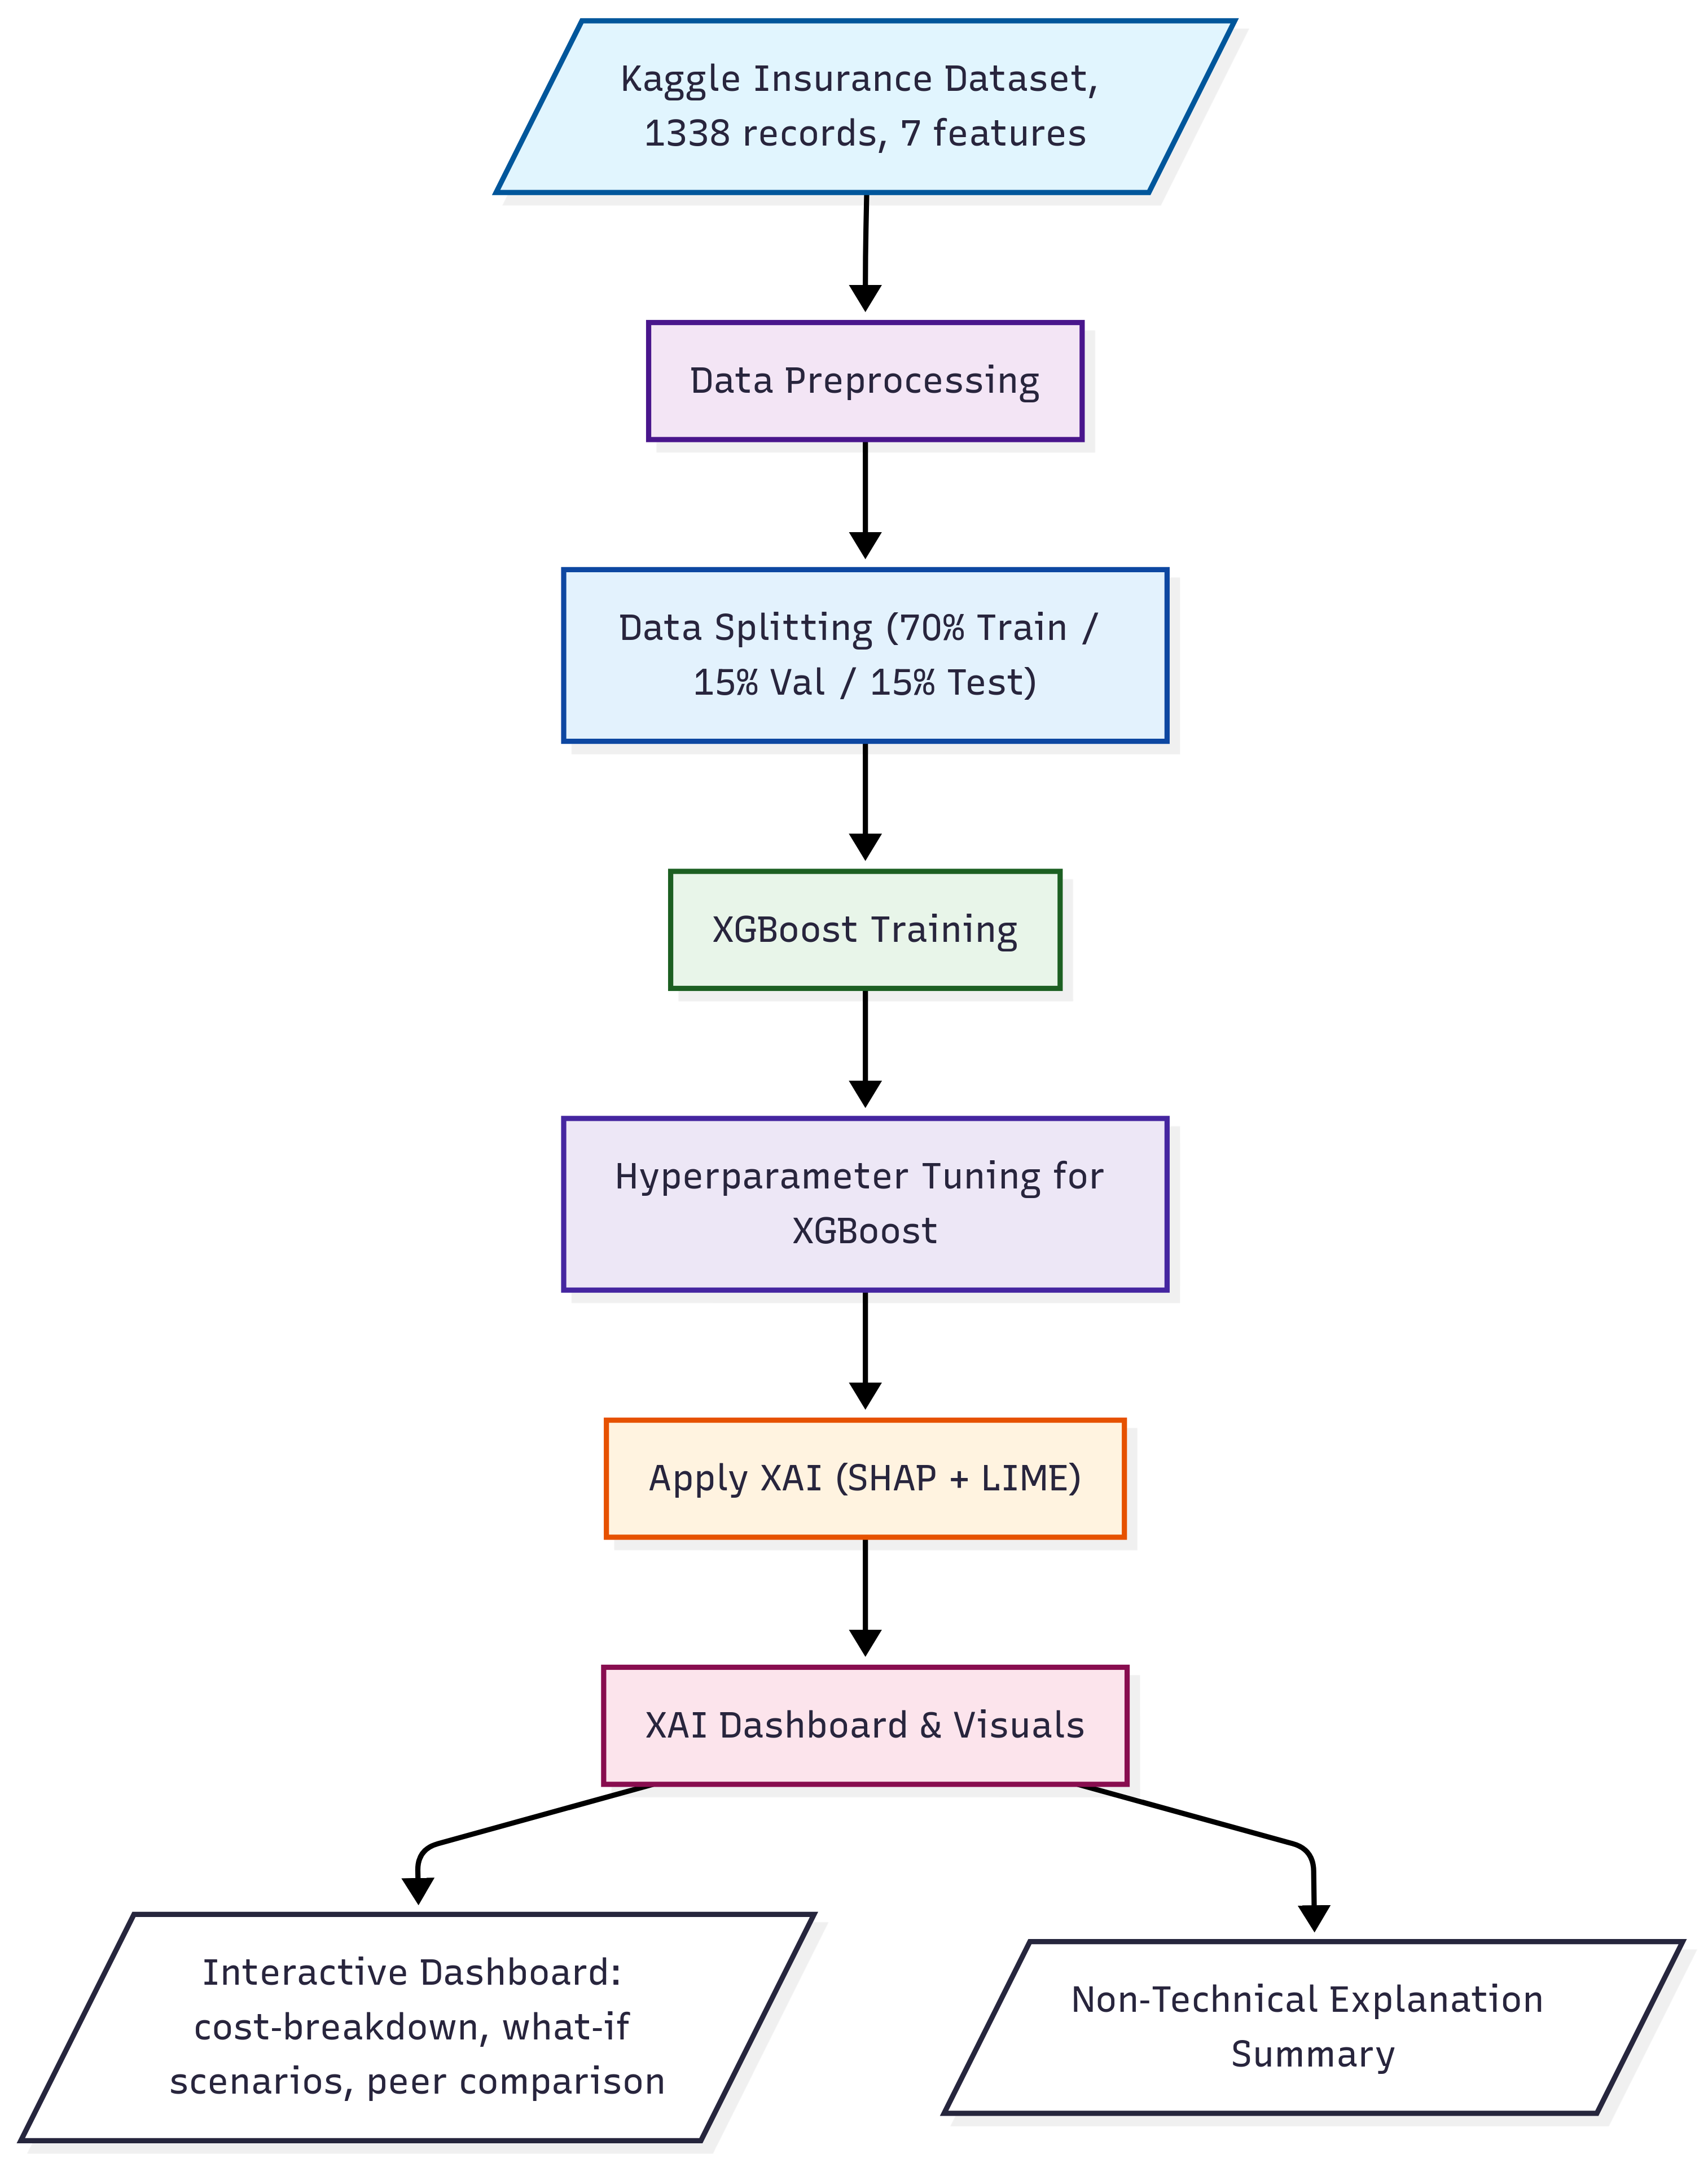
\includegraphics[width=0.9\textwidth]{XGBoost_XAI_Architecture.png}
  \caption{Arsitektur Sistem Prediksi Biaya Asuransi Kesehatan Berbasis XGBoost dengan Explainable AI}
  \label{fig:system_architecture}
\end{figure}

\section{Pengumpulan dan Preprocessing Data}

\subsection{Dataset Description}
Dataset Insurance Cost dari Kaggle berisi informasi 1338 individu dengan karakteristik:
\begin{itemize}
    \item \textbf{age}: Usia penerima manfaat utama (numerik, 18-64 tahun)
    \item \textbf{sex}: Jenis kelamin (kategorikal: female, male)
    \item \textbf{bmi}: Body Mass Index, kg/m² (numerik, 15.96-53.13)
    \item \textbf{children}: Jumlah tanggungan (numerik, 0-5)
    \item \textbf{smoker}: Status merokok (kategorikal: yes, no)
    \item \textbf{region}: Wilayah tempat tinggal di AS (kategorikal: northeast, southeast, southwest, northwest)
    \item \textbf{charges}: Biaya medis individual yang ditagihkan asuransi (target variable, numerik)
\end{itemize}

\subsection{Exploratory Data Analysis (EDA)}
EDA dilakukan untuk memahami karakteristik data dan mengidentifikasi pola yang relevan untuk XGBoost:
\begin{enumerate}
    \item \textbf{Distribusi Target Variable}: Analisis distribusi charges menunjukkan right-skewed distribution yang memerlukan transformation.
    \item \textbf{Feature Correlation Analysis}: Identifikasi korelasi untuk memahami feature interactions yang akan ditangkap XGBoost.
    \item \textbf{Categorical Feature Analysis}: Distribusi dan impact dari categorical variables terhadap charges.
    \item \textbf{Outlier Detection}: Identifikasi high-cost cases yang memerlukan special attention dalam modeling.
\end{enumerate}

\begin{algorithm}[H]
  \caption{Pipeline Preprocessing untuk XGBoost Implementation}
  \label{alg:preprocessing_xgboost}
  \DontPrintSemicolon
  \SetAlgoLined
  \SetKwProg{Fn}{Procedure}{:}{}
  \Fn{PreprocessForXGBoost($dataset$)}{
    \tcc{1. Handle Missing Values - XGBoost dapat handle internally}
    missing\_counts $\gets$ dataset.isnull().sum()\;
    \If{missing\_counts.any()}{
      \tcc{Mark missing values untuk XGBoost's built-in handling}
      dataset $\gets$ dataset.fillna(np.nan)\;
    }
    
    \tcc{2. Feature Engineering untuk Healthcare Context}
    dataset['age\_group'] $\gets$ pd.cut(dataset['age'], bins=[18,30,40,50,60,70])\;
    dataset['bmi\_category'] $\gets$ categorize\_bmi(dataset['bmi'])\;
    dataset['high\_risk'] $\gets$ (dataset['smoker'] == 'yes') \& (dataset['bmi'] > 30)\;
    dataset['family\_size'] $\gets$ dataset['children'] + 1\;
    
    \tcc{3. Encoding untuk XGBoost - Optimal untuk Tree-based}
    \ForEach{cat\_feature in ['sex', 'smoker']}{
      dataset[cat\_feature] $\gets$ LabelEncoder().fit\_transform(dataset[cat\_feature])\;
    }
    \tcc{One-hot encoding untuk region (low cardinality)}
    dataset $\gets$ pd.get\_dummies(dataset, columns=['region'], prefix='region')\;
    
    \tcc{4. Target Transformation untuk Skewed Distribution}
    dataset['log\_charges'] $\gets$ np.log1p(dataset['charges'])\;
    
    \tcc{5. Feature Scaling - Optional untuk XGBoost}
    \tcc{XGBoost is scale-invariant, but scaling helps SHAP interpretation}
    scaler $\gets$ StandardScaler()\;
    numeric\_features $\gets$ ['age', 'bmi', 'children']\;
    dataset[numeric\_features] $\gets$ scaler.fit\_transform(dataset[numeric\_features])\;
    
    \Return dataset, scaler\;
  }
\end{algorithm}

\subsection{Data Splitting Strategy}
Dataset dibagi dengan stratified sampling untuk mempertahankan distribusi charges:
\begin{itemize}
    \item \textbf{Training Set}: 70\% (936 records) - untuk training XGBoost
    \item \textbf{Validation Set}: 15\% (201 records) - untuk hyperparameter tuning
    \item \textbf{Test Set}: 15\% (201 records) - untuk final evaluation
\end{itemize}

\section{Implementasi dan Optimasi XGBoost}

\subsection{Baseline Model}
Linear Regression diimplementasikan sebagai baseline untuk mendemonstrasikan improvement dari XGBoost:

\begin{algorithm}[H]
  \caption{Baseline Linear Regression Implementation}
  \label{alg:baseline_lr}
  \DontPrintSemicolon
  \SetAlgoLined
  \SetKwProg{Fn}{Function}{:}{}
  \Fn{TrainBaselineModel($X_{train}$, $y_{train}$)}{
    \tcc{Simple Linear Regression sebagai baseline}
    lr\_model $\gets$ LinearRegression()\;
    lr\_model.fit($X_{train}$, $y_{train}$)\;
    
    \tcc{Calculate baseline metrics}
    baseline\_pred $\gets$ lr\_model.predict($X_{train}$)\;
    baseline\_r2 $\gets$ r2\_score($y_{train}$, baseline\_pred)\;
    baseline\_rmse $\gets$ sqrt(mean\_squared\_error($y_{train}$, baseline\_pred))\;
    
    \Return lr\_model, baseline\_r2, baseline\_rmse\;
  }
\end{algorithm}

\subsection{XGBoost Implementation}
Implementasi XGBoost dengan careful configuration untuk healthcare data:

\begin{algorithm}[H]
  \caption{XGBoost Implementation untuk Healthcare Cost Prediction}
  \label{alg:xgboost_implementation}
  \DontPrintSemicolon
  \SetAlgoLined
  \SetKwProg{Fn}{Function}{:}{}
  \Fn{ImplementXGBoost($X_{train}$, $y_{train}$, $X_{val}$, $y_{val}$)}{
    \tcc{1. Initial XGBoost Configuration}
    base\_params $\gets$ \{
      'objective': 'reg:squarederror',
      'eval\_metric': ['rmse', 'mae'],
      'tree\_method': 'hist',  // Faster for larger datasets
      'enable\_categorical': True,  // Native categorical support
      'random\_state': 42
    \}\;
    
    \tcc{2. Hyperparameter Search Space}
    param\_grid $\gets$ \{
      'n\_estimators': [100, 200, 300, 500],
      'max\_depth': [3, 4, 5, 6, 7],
      'learning\_rate': [0.01, 0.05, 0.1, 0.15],
      'subsample': [0.6, 0.7, 0.8, 0.9],
      'colsample\_bytree': [0.6, 0.7, 0.8, 0.9],
      'reg\_alpha': [0, 0.01, 0.1, 1],
      'reg\_lambda': [0.1, 1, 2, 5],
      'min\_child\_weight': [1, 3, 5, 7]
    \}\;
    
    \tcc{3. Randomized Search with Cross-Validation}
    xgb\_model $\gets$ XGBRegressor(**base\_params)\;
    
    random\_search $\gets$ RandomizedSearchCV(
      estimator=xgb\_model,
      param\_distributions=param\_grid,
      n\_iter=100,  // Number of parameter combinations
      cv=5,  // 5-fold cross-validation
      scoring='neg\_mean\_squared\_error',
      n\_jobs=-1,
      verbose=1,
      random\_state=42
    )\;
    
    \tcc{4. Fit with Early Stopping}
    eval\_set $\gets$ [($X_{train}$, $y_{train}$), ($X_{val}$, $y_{val}$)]\;
    
    random\_search.fit(
      $X_{train}$, $y_{train}$,
      eval\_set=eval\_set,
      early\_stopping\_rounds=20,
      verbose=False
    )\;
    
    \tcc{5. Extract Best Model and Parameters}
    best\_model $\gets$ random\_search.best\_estimator\_\;
    best\_params $\gets$ random\_search.best\_params\_\;
    
    \Return best\_model, best\_params\;
  }
\end{algorithm}

\subsection{Feature Importance Analysis}
Native XGBoost feature importance untuk initial understanding:

\begin{algorithm}[H]
  \caption{XGBoost Feature Importance Extraction}
  \label{alg:feature_importance}
  \DontPrintSemicolon
  \SetAlgoLined
  \SetKwProg{Fn}{Function}{:}{}
  \Fn{AnalyzeFeatureImportance($xgb\_model$, $feature\_names$)}{
    \tcc{Get multiple importance types}
    importance\_types $\gets$ ['weight', 'gain', 'cover']\;
    importance\_dict $\gets$ \{\}\;
    
    \ForEach{imp\_type in importance\_types}{
      importance $\gets$ xgb\_model.get\_booster().get\_score(importance\_type=imp\_type)\;
      importance\_dict[imp\_type] $\gets$ importance\;
    }
    
    \tcc{Create importance dataframe}
    feature\_imp\_df $\gets$ pd.DataFrame(importance\_dict)\;
    feature\_imp\_df['feature'] $\gets$ feature\_names\;
    feature\_imp\_df $\gets$ feature\_imp\_df.sort\_values('gain', ascending=False)\;
    
    \tcc{Visualize importance}
    plot\_importance(xgb\_model, importance\_type='gain', max\_num\_features=10)\;
    
    \Return feature\_imp\_df\;
  }
\end{algorithm}

\section{Integrasi Explainable AI}

\subsection{SHAP Implementation untuk XGBoost}
TreeSHAP provides exact Shapley values untuk XGBoost:

\begin{algorithm}[H]
  \caption{SHAP Integration dengan XGBoost}
  \label{alg:shap_xgboost}
  \DontPrintSemicolon
  \SetAlgoLined
  \SetKwProg{Fn}{Function}{:}{}
  \Fn{ImplementSHAP($xgb\_model$, $X$, $feature\_names$)}{
    \tcc{1. Initialize TreeSHAP Explainer}
    explainer $\gets$ shap.TreeExplainer(
      xgb\_model,
      feature\_perturbation='tree\_path\_dependent'
    )\;
    
    \tcc{2. Calculate SHAP Values}
    shap\_values $\gets$ explainer.shap\_values($X$)\;
    expected\_value $\gets$ explainer.expected\_value\;
    
    \tcc{3. Global Feature Importance}
    global\_importance $\gets$ np.abs(shap\_values).mean(axis=0)\;
    importance\_df $\gets$ pd.DataFrame(\{
      'feature': feature\_names,
      'importance': global\_importance
    \}).sort\_values('importance', ascending=False)\;
    
    \tcc{4. Generate Visualizations}
    \tcc{Summary plot untuk global understanding}
    shap.summary\_plot(shap\_values, $X$, feature\_names=feature\_names)\;
    
    \tcc{Dependence plots untuk top features}
    top\_features $\gets$ importance\_df['feature'].head(4)\;
    \ForEach{feature in top\_features}{
      shap.dependence\_plot(feature, shap\_values, $X$, feature\_names=feature\_names)\;
    }
    
    \tcc{5. Individual Explanations}
    \ForEach{idx in sample\_indices}{
      \tcc{Waterfall plot untuk individual prediction}
      shap.waterfall\_plot(shap.Explanation(
        values=shap\_values[idx],
        base\_values=expected\_value,
        data=$X$.iloc[idx],
        feature\_names=feature\_names
      ))\;
    }
    
    \Return shap\_values, expected\_value, importance\_df\;
  }
\end{algorithm}

\subsection{LIME Implementation untuk Patient-Facing Explanations}
LIME untuk quick, intuitive explanations:

\begin{algorithm}[H]
  \caption{LIME Implementation untuk XGBoost}
  \label{alg:lime_xgboost}
  \DontPrintSemicolon
  \SetAlgoLined
  \SetKwProg{Fn}{Function}{:}{}
  \Fn{ImplementLIME($xgb\_model$, $X_{train}$, $X_{test}$, $feature\_names$)}{
    \tcc{1. Initialize LIME Explainer}
    explainer $\gets$ lime.lime\_tabular.LimeTabularExplainer(
      training\_data=$X_{train}$.values,
      feature\_names=feature\_names,
      mode='regression',
      discretize\_continuous=True  // Better untuk patient understanding
    )\;
    
    \tcc{2. Generate Explanations untuk Test Samples}
    lime\_explanations $\gets$ []\;
    
    \ForEach{idx in range(len($X_{test}$))}{
      \tcc{Explain individual instance}
      exp $\gets$ explainer.explain\_instance(
        $X_{test}$.iloc[idx].values,
        xgb\_model.predict,
        num\_features=6,  // Top 6 features
        num\_samples=5000  // Sampling untuk local approximation
      )\;
      
      \tcc{Extract explanation data}
      exp\_dict $\gets$ \{
        'prediction': xgb\_model.predict([$X_{test}$.iloc[idx]])[0],
        'explanation': exp.as\_list(),
        'local\_pred': exp.local\_pred[0],
        'score': exp.score
      \}\;
      
      lime\_explanations.append(exp\_dict)\;
    }
    
    \tcc{3. Generate Visualizations}
    \ForEach{exp in lime\_explanations[:5]}{  // First 5 samples
      exp.as\_pyplot\_figure()\;
    }
    
    \Return lime\_explanations\;
  }
\end{algorithm}

\subsection{Comparative Analysis: SHAP vs LIME}
Systematic comparison untuk optimal usage:

\begin{table}[h]
  \centering
  \caption{SHAP vs LIME Comparison untuk XGBoost Explanations}
  \label{tab:shap_lime_comparison}
  \begin{tabular}{|l|l|l|}
    \hline
    \textbf{Aspect} & \textbf{SHAP} & \textbf{LIME} \\
    \hline
    Computation Time & O(TLD²) - Slower & O(N) - Faster \\
    \hline
    Accuracy & Exact Shapley values & Local approximation \\
    \hline
    Global Insights & Excellent & Limited \\
    \hline
    Patient Understanding & Technical & Intuitive \\
    \hline
    Best Use Case & Regulatory/Clinical & Patient Interface \\
    \hline
  \end{tabular}
\end{table}

\section{Patient-Centric Framework Development}

\subsection{Design Principles}
Framework dirancang dengan prinsip patient empowerment:
\begin{enumerate}
    \item \textbf{Clarity}: Penjelasan dalam bahasa non-technical
    \item \textbf{Interactivity}: User dapat explore different scenarios
    \item \textbf{Actionability}: Insights mengarah pada concrete actions
    \item \textbf{Personalization}: Tailored untuk individual circumstances
\end{enumerate}

\subsection{Dashboard Architecture}

\begin{algorithm}[H]
  \caption{Patient-Centric Dashboard Implementation}
  \label{alg:dashboard}
  \DontPrintSemicolon
  \SetAlgoLined
  \SetKwFunction{Fn}{Function}
  \Fn{BuildPatientDashboard(xgb\_model, shap\_explainer, lime\_explainer)}{
    \tcc{1. Initialize Dashboard Components}
    dashboard $\gets$ \{
      'prediction\_module': PredictionEngine($xgb\_model$),
      'shap\_module': SHAPVisualizer($shap\_explainer$),
      'lime\_module': LIMEInterface($lime\_explainer$),
      'whatif\_module': WhatIfAnalyzer($xgb\_model$),
      'narrative\_module': NarrativeGenerator()
    \}\;
    
    \tcc{2. Prediction Module}
    \Fn{PredictCost($patient\_data$)}{
      prediction $\gets$ xgb\_model.predict($patient\_data$)\;
      confidence\_interval $\gets$ calculate\_prediction\_interval(prediction)\;
      \Return prediction, confidence\_interval\;
    }
    
    \tcc{3. Explanation Module}
    \Fn{GenerateExplanation($patient\_data$, $method$='hybrid')}{
      \If{method == 'detailed'}{
        explanation $\gets$ shap\_explainer.explain($patient\_data$)\;
      }
      \ElseIf{method == 'quick'}{
        explanation $\gets$ lime\_explainer.explain($patient\_data$)\;
      }
      \Else{  // Hybrid approach
        shap\_exp $\gets$ shap\_explainer.explain($patient\_data$)\;
        lime\_exp $\gets$ lime\_explainer.explain($patient\_data$)\;
        explanation $\gets$ combine\_explanations(shap\_exp, lime\_exp)\;
      }
      \Return explanation\;
    }
    
    \tcc{4. What-If Analysis}
    \Fn{WhatIfScenario($patient\_data$, $changes$)}{
      scenarios $\gets$ []\;
      \ForEach{change in changes}{
        modified\_data $\gets$ apply\_change($patient\_data$, change)\;
        new\_prediction $\gets$ xgb\_model.predict(modified\_data)\;
        impact $\gets$ new\_prediction - original\_prediction\;
        scenarios.append(\{change, new\_prediction, impact\})\;
      }
      \Return scenarios\;
    }
    
    \tcc{5. Narrative Generation}
    \Fn{GenerateNarrative($prediction$, $explanation$, $patient\_data$)}{
      narrative $\gets$ []\;
      narrative.append(f"Estimasi biaya asuransi Anda: \${prediction:.2f}")\;
      
      \tcc{Top factors affecting cost}
      top\_factors $\gets$ get\_top\_factors($explanation$, n=3)\;
      \ForEach{factor in top\_factors}{
        impact\_text $\gets$ describe\_impact(factor)\;
        narrative.append(impact\_text)\;
      }
      
      \tcc{Actionable recommendations}
      recommendations $\gets$ generate\_recommendations(top\_factors, $patient\_data$)\;
      narrative.extend(recommendations)\;
      
      \Return " ".join(narrative)\;
    }
    
    \Return dashboard\;
  }
  
\end{algorithm}

\subsection{Interactive Visualizations}
Visualizations designed untuk patient understanding:
\begin{enumerate}
    \item \textbf{Cost Breakdown Pie Chart}: Shows percentage contribution of each factor
    \item \textbf{Feature Impact Bar Chart}: Positive/negative impacts on cost
    \item \textbf{What-If Sliders}: Interactive exploration of scenarios
    \item \textbf{Peer Comparison}: Anonymous comparison dengan similar demographics
    \item \textbf{Trend Projections}: Future cost estimates based on age progression
\end{enumerate}

\section{Evaluasi Sistem}

\subsection{Performance Metrics}
Evaluasi komprehensif XGBoost performance:

\begin{table}[h]
  \centering
  \caption{Evaluation Metrics untuk XGBoost Performance}
  \label{tab:evaluation_metrics}
  \begin{tabular}{|l|l|l|}
    \hline
    \textbf{Metric} & \textbf{Formula} & \textbf{Target} \\
    \hline
    R² Score & $1 - \frac{\sum(y_i - \hat{y}_i)^2}{\sum(y_i - \bar{y})^2}$ & > 0.85 \\
    \hline
    RMSE & $\sqrt{\frac{1}{n}\sum(y_i - \hat{y}_i)^2}$ & Minimize \\
    \hline
    MAE & $\frac{1}{n}\sum|y_i - \hat{y}_i|$ & Minimize \\
    \hline
    MAPE & $\frac{100}{n}\sum|\frac{y_i - \hat{y}_i}{y_i}|$ & < 15\% \\
    \hline
  \end{tabular}
\end{table}

\subsection{XAI Effectiveness Evaluation}
Metrics untuk evaluating explanation quality:
\begin{itemize}
    \item \textbf{Consistency}: Agreement antara SHAP dan LIME rankings
    \item \textbf{Stability}: Variation in explanations dengan different samples
    \item \textbf{Comprehensibility}: User understanding scores (simulated)
    \item \textbf{Computational Efficiency}: Time untuk generate explanations
\end{itemize}

\subsection{System Usability Testing}
Framework evaluation dari patient perspective:
\begin{enumerate}
    \item Response time untuk predictions
    \item Clarity of explanations
    \item Usefulness of what-if scenarios
    \item Overall user satisfaction (simulated metrics)
\end{enumerate}

\section{Ethical Considerations}

\subsection{Data Privacy}
\begin{itemize}
    \item Dataset adalah publicly available dan anonymized
    \item Tidak ada informasi pribadi yang dapat diidentifikasi (PII)
    \item Compliance dengan research ethics guidelines
\end{itemize}

\subsection{Model Fairness}
\begin{itemize}
    \item Analysis untuk demographic bias dalam predictions
    \item Fair representation across regions dan demographics
    \item Transparent reporting of model limitations
\end{itemize}

\subsection{Patient Autonomy}
\begin{itemize}
    \item Predictions presented sebagai estimates dengan confidence intervals
    \item Clear disclaimers tentang model limitations
    \item Emphasis pada informed decision-making, bukan prescriptive advice
\end{itemize}